\chapter{Cloud Security with Honeypots}

In this chapter we investigate... tbc.
In \fullref{sec:honeypots-heicloud}, we show various results of honeypots in heiCLOUD, stress out the importance of it, and lay emphasis on our concept in \autoref{chap:concept}.

\section{Introduction}

As previously mention in \fullref{sec:cloud-computing}, using cloud resources are becoming the go-to option for new services, and applications.
\citet{Kelly2021} thoroughly investigated honeypots on cloud providers such as Azure, AWS, or Goolge Cloud Platform.
Followingly, we present their results that we want to compare with the results of HeiCLOUD later on.
The results are collected by T-Pot version $20.06.0.$ over a duration of 3 weeks.
A detailed description of T-Pot is done in \fullref{sec:tpot}.
In addition, \citet{Kelly2021} considered different server geographical locations.
They have collected data from East US, West Europe, Southeast Asia.
\autoref{tab:overview-cloud-security} shows the results presented by \citet{Kelly2021}.
Dionaea, Cowire, and Conpot are the most attacked honeypots in comparison to the others.
Regarding \ac{aws}, Dionaea account $91\%$ of the total attacks, Glutton and Cowire are minor with $5\%$, and $2\%$.
Interestingly, Cowire reported several attacks related to the COVID-19 pandamic to enable social engineering methods.
In contrast to \ac{aws}, Cowire logged the majority of attacks with $51\%$ on \ac{gc}.
Beside several automated attacks trying to login with default credentials, adversaries tried to gather information about CPU architecture, scheduled tasks, and privilege escalation.
Microsoft Azure reflects nearly the same results as the other two cloud providers beforehand.

\begin{table}
    \centering
    \caption[Overview of attacks on cloud providers]{Overview of attacks on cloud providers. For a better overview, only the three most attacked honeypots are listed. The others combine several honeypots.}
    \begin{tabular}{l|llll|l}
        \toprule
        \textbf{Provider} & \multicolumn{4}{c|}{\textbf{Honeypot}} & \textbf{In Total}                                   \\
                          & Dionaea                                & Cowire            & Glutton  & others   &           \\
        \hline
        \acl{aws}         & $228.075$                              & $4.503$           & $11.878$ & $3.688$  & $248.144$ \\
        \acl{gc}          & $162.570$                              & $297.818$         & $84.375$ & $36.403$ & $581.116$ \\
        Microsoft Azure   & $308.102$                              & $9.012$           & $17.256$ & $6.365$  & $340.735$ \\
        \bottomrule
    \end{tabular}
    \label{tab:overview-cloud-security}
\end{table}

The overall results show an average ratio of $55.000$ attacks per day, summing up to roughly $1.6$ mio in total.
Similar results for different regions could have been reprocuded.
Their results clearly show the disparty of the regions Europe, US, and Asia.
An important question that \citet{Kelly2021} answered is if attackers target services on cloud providers based on the cloud providers' market share.
They could not confirm this assumption based on the fact that Google Cloud with the smallest market share received most of the attacks.
In total, the most of the attacks are originated from Vietnam, Russia, United States, and China.
Due to technologies such as VPN, or Tor, the geolocation only indicates the last node, so location data might be distored.
Across all providers roughly $80\%$ of the source IP addresses had a bad reputation and could been filtered by the organization.
The operating devices used for attacking the services are mostly Windows 7 or 8, and different Linux kernels and distros.
Windows devices target vulnerabilities in remote desktop sharing software. Such vulnerabilities are
\begin{enumerate*}[label=(\roman*)]
    \item CVE-2006-2369\cite{CVE-2006-2369} (RealVNC) in the US region,
    \item CVE-2001-0540\cite{CVE-2001-0540} (RDP) in EU and Asia regions,
    \item CVE-2012-0152\cite{CVE-2012-0152} (RDP) in the Asia region, and
    \item CVE-2005-4050\cite{CVE-2005-4050} (VoIP) in EU region
\end{enumerate*}.
In addition, attackers were also capable of disguising any fingerprinting activity of p0f.

In this chapter, we want to compare the findings \citet{Kelly2021} claimed in the paper \enquote{A Comparative Analysis of Honeypots on Different
    Cloud Platforms} with ours using the University Heidelberg's cloud solution.
First, a short introduction of heiCLOUD is held, followed by a closer lookup of T-Pot that is used to acquire data.
Lastly, we present the results and do a thorough comparison.

\section{Methodology}

\subsection{Cloud Provider}

\citet{urz2021} offers a \enquote{\ac{iaas} specially tailored for higher education and research institutions} called heiCLOUD.
It supplies multiple institutes at University Heidelberg with storage, virtual machines, or network components.
In addition, heiCLOUD is a DFN\footnote{German National Research and Education Network,  the communications network for Science and research in Germany} member, and offers others to use their services.
As stated on their information website\cite{heicloud2021}, it is
\begin{enumerate*}[label=(\roman*)]
    \item capable of freely manageable IT resources,
    \item beholds a stable and fast connection,
    \item ensures high availability and scalability,
    \item has freely selectable VM operating systems, and
    \item has a transparent payment model
\end{enumerate*} \cite{heicloud2021}.
Based on the open source application OpenStack, users can easily create own network areas, and manage their space individually.
Unlike well-known cloud providers, heiCLOUD servers are located withing Germany, thus, abide by the European data privacy law.
HeiCLOUD have never considered honeypots for additional cyber security measurements.

\subsection{T-Pot}
\label{sec:tpot}

To be able to compare our results with \citet{Kelly2021}, we use the same approach to capture recent cyber attacks.
The T-Pot solution, a mixture of Telekom and Honeypot, stands out with their sheer quantity of various honeypots.
It requires $8$ GB RAM and a minimum of $128$ GB hard drive storage.
Based on a Debian 10 Buster distribution, it relies on Docker to run their services \cite{combe2016}.
T-Pot has to be deployed in a reachable network where intruders are expected.
Either TCP and UDP traffic are forwarded without filtering to the network interface, or run it behind a firewall with forwarding rules.
Specifified ports for attackers are $1$-$64000$, higher ports are reserved for trusted IPs, thus, a reverse proxy checks basic authentication.
All daemons and tools run on the same network interface whereas some of them are encapsulated in their own Docker network.
Docker is a lightweight virtualization technology that uses containers to run on the host system.
More to docker...
\autoref{fig:overview-tpot} visualizes the technical concept of T-Pot.
Each service has dedicated ports or port ranges that are exposed.
Attackers can send TCP or UDP packets.
...More about the technical concept.
In addition, T-Pot features different services types, namely
\begin{enumerate*}[label=(\roman*)]
    \item standard,
    \item sensor,
    \item industrial,
    \item collector,
    \item next generation, and
    \item medical
\end{enumerate*}.
Each service type features a different set of honeypots and tools tailored to their core idea.
T-Pot feeds their data to an external Telekom service, however, this data submission can be turned off.
For this chapter we restrict ourself to the latest version $20.06.0$.
Newer versions might be available by time and could differ from ours.

\begin{sidewaysfigure}
    \centering
    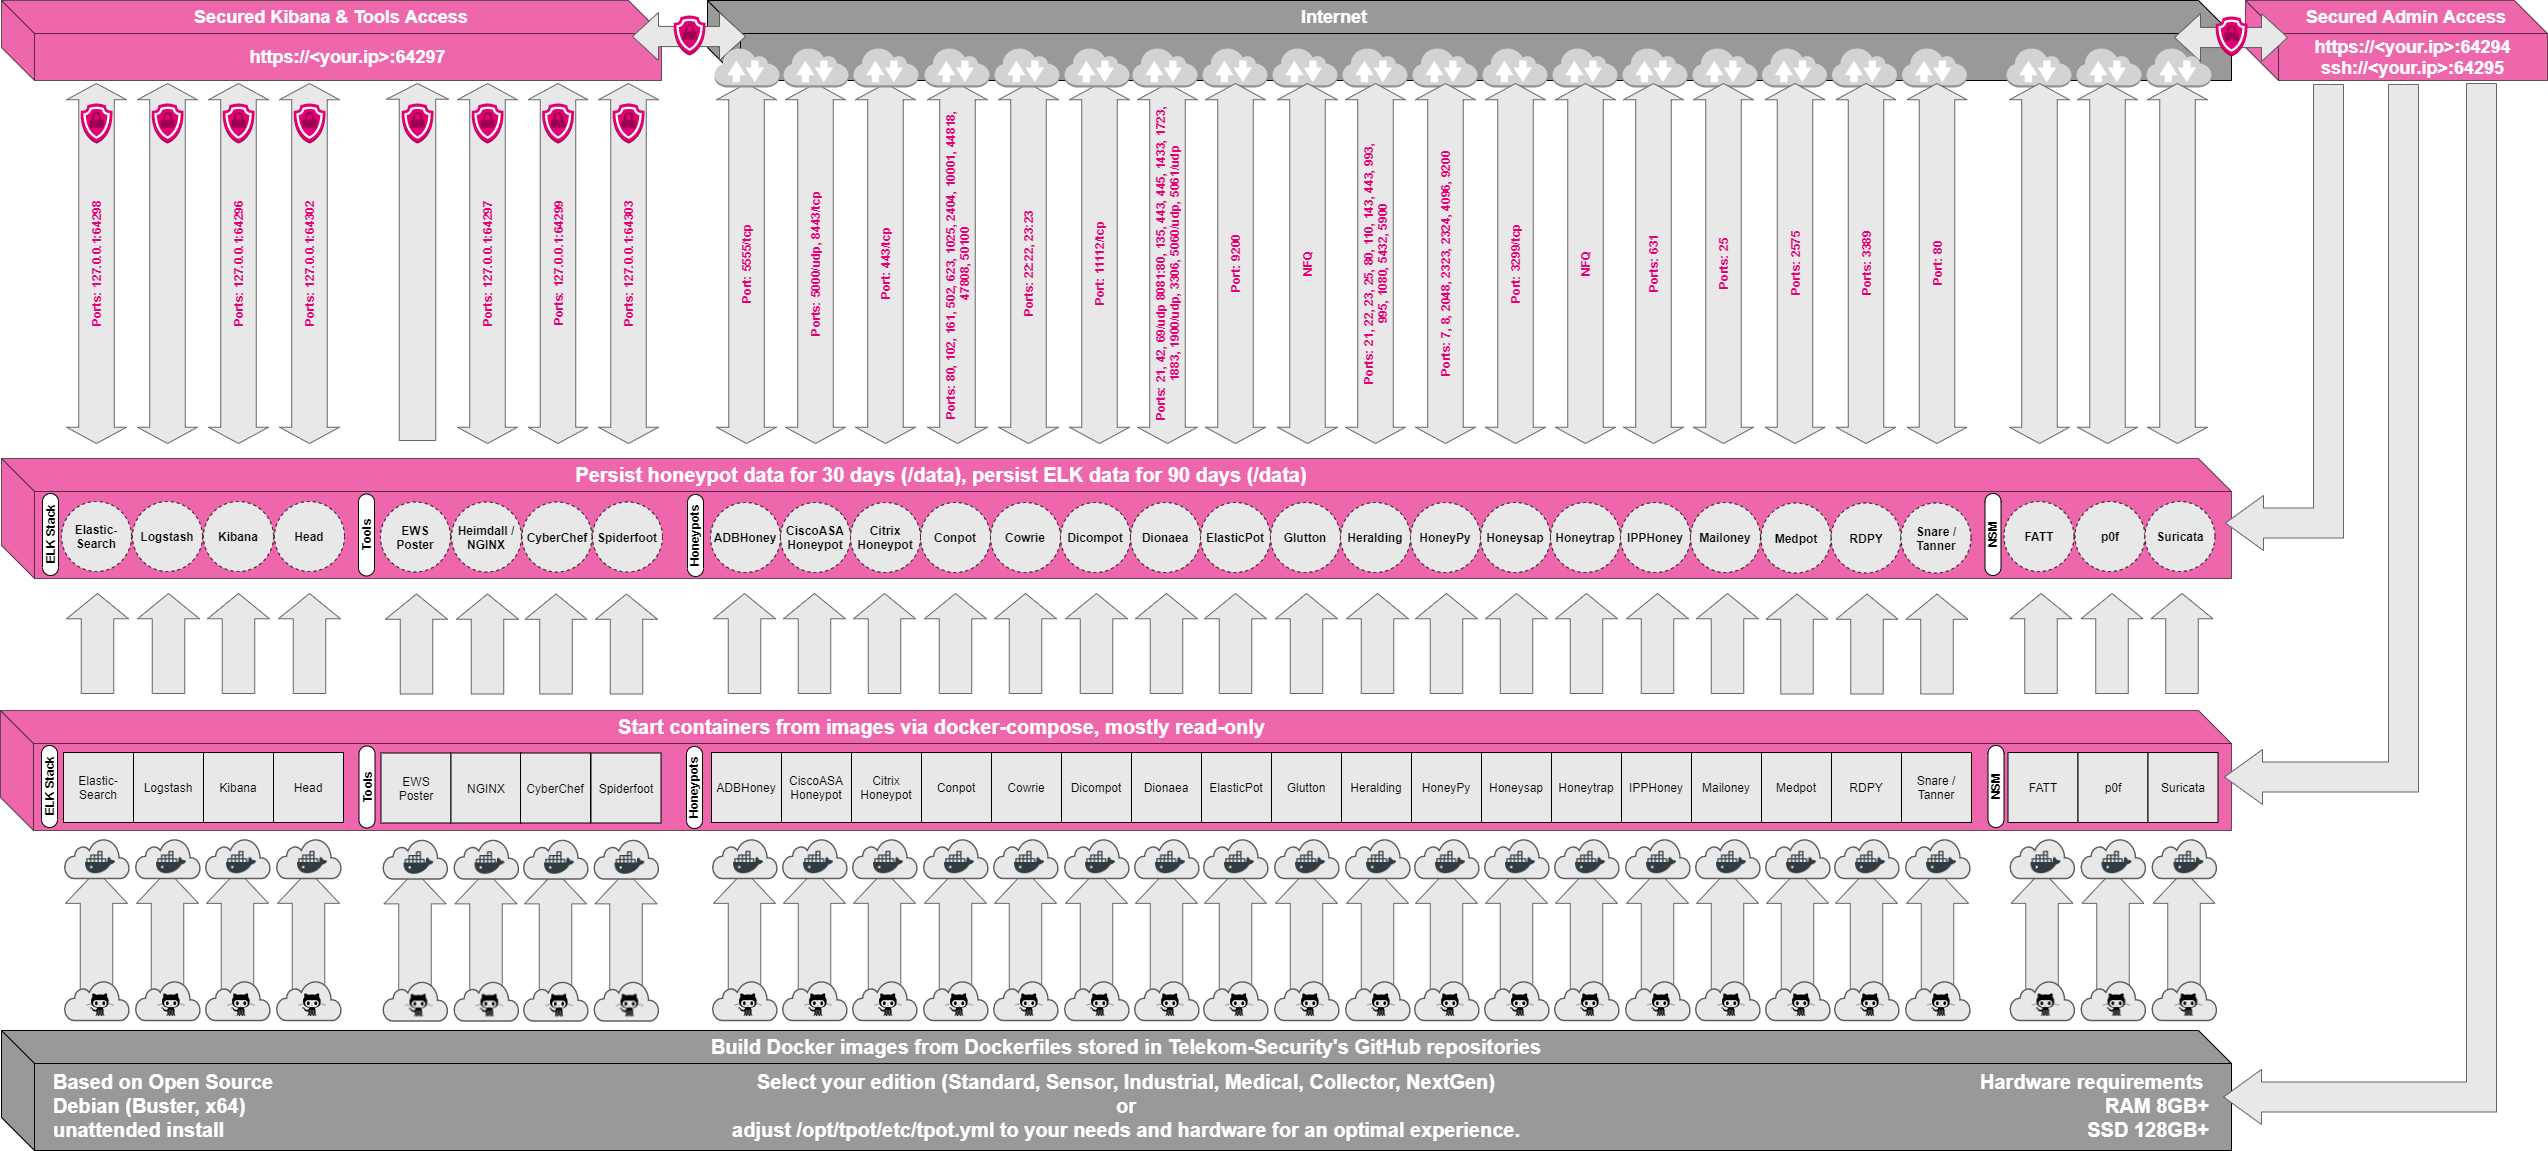
\includegraphics[width=\textwidth]{figures/architecture.png}
    \caption{}
    \label{fig:overview-tpot}
\end{sidewaysfigure}

\subsubsection{Honeypots}

T-Pot combines honeypots with several tools to get a deeper inside of attackers.
Followingly, all available components will be explained, albeit the sheer quantity of it.
In addition, \autoref{tab:overview-honeypots} gives a quick overview of all available honeypots in conjunction with
\begin{enumerate*}[label=(\roman*)]
    \item the port they are running on,
    \item what service type they are,
    \item what kind of interaction level, and
    \item a short decription
\end{enumerate*}.

\textbf{ADBHoney} \cite{adbhoney2021} is a low interaction \ac{adb} honeypot over TCP/IP.
The importance of it lies in the \ac{adb} protocol that is used to debug and push content to the device.
However, unlike USB it does not support any kind of ample mechanisms of authentication and protection.
By exposing the \ac{adb} service over any port, an adversary could connect and exploit it.
ADBHoney is designed to catch malware that has been pushed onto devices.

\textbf{Cisco \ac{asa}} \cite{cymmetria2018} is a low interaction honeypot that detects CVE-2018-0101\cite{CVE-2018-0101}.
It is a vulnerability that could allow an unauthenticated, remote attacker to cause a reload of the affected system or to remotely execute code.
This can be achieved by flooding a webvpn-configured interface with crafted XML packets.
Consequently, the attacker obtain full control by executing arbitrary code.

\textbf{Citrix \ac{adc} honeypot} \cite{citrixhoneypot2020} detects and logs CVE-2019-19781\cite{CVE-2019-19781} scans and exploitation attempts.
This vulnerability allows adversaries to perform directory traversal attacks.
Files are accessible by path strings to denote the file or directory.
In addition, some file systems include special character to easily traverse the hierarchy.
Attackers take advantage of it by combining special characters in order to get access to restricted areas. \cite{flanders2019}

\textbf{Conpot} \cite{conpot2021} is a low interaction industrial honeypot for \ac{ics}, and \ac{scada}.
It provides a variety of different common industrial control protocols.
An adversary should be tricked by the complex infrastructure, and lure him into attacks.
In addition, a custom human machine interface can be conntected to increase the attack surface.
By randomly delaying the response time, conpot tries to emulate a real machine handling a certain amount of load.

\textbf{Cowrie} \cite{cowire2021} is a medium to high interaction SSH and Telnet honeypot.
It offers to log brute-force attacks and shell interactions with attacker.
In medium interaction mode cowire emulates a UNIX shell in Python, whereas in high interaction mode it proxies all commands to another system.

\textbf{DDoSPot} \cite{ddosspot2021} is a low interaction honeypot to log and detect UDP-based \ac{ddos} attacks.
It is used as a platform to support various plugins for different honeypot services, and servers.
Currently, it supports DNS, NTP, SSDP, CHARGEN, and random/mock UDP server.

\textbf{Dicompot} \cite{dicompot2021} is a low interaction honeypot for the \ac{dicom} protocol.
As other honeypots before, it mocks a \ac{dicom} server in Go to collect logs and detect attacks.

\textbf{Dionaea} \cite{dionaea2021} is a medium interaction honeypot that tries to capture malware copies by exposing services.
It supports a vast variety of protocols such as FTP, SMB, and HTTP.
Several modules can be integrated to work with Dionaea such as VirusTotal for further malware results.

\textbf{Elasticpot} \cite{elasticpot2021} is a low interaction honeypot for elasticsearch, a search engine based on the Lucene library.

\textbf{Glutton} \cite{glutton2021} is a generic low interaction honeypot that works as a MitM for SSH and TCP.
However, lacking documentation does not provide a deeper inside of this honeypot.

\textbf{Heralding} \cite{heralding2021} is a credential catching honeypot for protocols like FTP, Telnet, SSH, HTTP, or IMAP.

\textbf{HoneyPy} \cite{honeysap2021} is a low to medium interaction honeypot that supports several protocols such as UDP, or TCP.
New protocols can be added by writing a custom plugin for it.
HoneyPy should give the freedom of easily deploying and extending honeypots.

\textbf{HoneySAP} \cite{honeysap2021} is a low interaction honeypot tailored for SAP services.

\textbf{HoneyTrap} \cite{honeytrap2021} is a low interaction honeypot network security tool.
As stated by \citet*{honeytrap2021}, HoneyTrap is vulnerable to buffer overflow attacks.

\textbf{IPPHoney} \cite{ipphoney2021} is a low interaction \ac{ipp} honeypot.

\textbf{Mailoney} is a low interaction SMTP honeypot written in Python.

\textbf{MEDpot} \cite{medpot2021} is a low interaction honeypot focused on \ac{fhir}.
It is a standard decription data format to transfer and exchange medical health records.

\textbf{RDPY} \cite{rdpy2021} is a low interaction honeypot of the Microsoft \ac{rdp} written in Python.
It features client and server side, and it based on the event driven network engine Twisted.
It supports authentication over SSL and NLA.

\textbf{SNARE and TANNER} \cite{snare2021, tanner2021} is a honeypot project.
SNARE is an abbreviation for Super Next generation Advanced Reactive honEypot.
It is a successor of Glastopf, a web application sensor.
In addition, it supports the feature of converting existing webpages into attack surfaces.
TANNER \cite{tanner2021} can be seen as SNARES's brain.
Whenever a request has been sent to SNARE, TANNER decides how the response should like.

\subsubsection{Tools}

In addition, T-Pot integrates following tools to investigate and handle network traffic. Followingly, we investigate the most important ones:

\textbf{FATT}\cite{fatt2021} is used to extract metadata and fingerprints such as JA3\cite{ja32021} and HASSH\cite{hassh2021} from captured packets.
JA3 is a method for \enquote{creating SSL/TLS client fingerprints} whereas HASSH is a \enquote{network fingerprinting standard which can be used to identify specific client and server SSH implementations}.
In addition, it features live network traffic.
As noted by the author, Fatt is based on a python wrapper for tshark, namely pyshark, and thus having performance downturns.

\textbf{Spiderfoot}

\textbf{Suricata}

\textbf{p0f}

\textbf{Endlessh} \cite{endlessh2021} is a SSH server that sends an endless, random SSH banner.
The key idea is to lock up SSH clients that try to connect to the SSH server.
It lowers the transcation speed by intentionally inserting delays.
Due to connection establishing before cryptographic exchange, this module does not require any cryptographic libraries.

\textbf{HellPot} \cite{hellpot2021} is a \enquote{endless honeypot}.
Connecting to this honeypot results in a memory overflow.
Its key idea is to send an endless stream of data to the attacker until its memory, or storage runs out.


\begin{sidewaystable}
    \centering
    \caption[Overview honeypots of T-Pot]{Overview of all available honeypots and tools of T-Pot with interaction level, port, and a short description. Ports are marked with either TCP or UDP, if a port misses any definition, both TCP and UDP are allowed.}
    \resizebox{1\textwidth}{!}{%
    \begin{tabularx}{\linewidth}{l|XlX}
        \toprule
        \textsc{Honeypots}                       & \multicolumn{3}{c}{}                                                                                                                                                                                                            \\
                                                 & \textbf{Port}                                                                                               & \textbf{Interaction-level} & \textbf{Description}                                                                 \\
        \hline
        adbhoney \cite{adbhoney2021}             & 5555/tcp                                                                                                    & low                        & \ac{adb} protocol honeypot                                                           \\
        ciscoasa \cite{cymmetria2018}            & 5000/udp, 8443/tcp                                                                                          & low                        & honeypot for CVE-2018-0101\cite{CVE-2018-0101} detection                             \\
        citrixhoneypot \cite{citrixhoneypot2020} & 443/tcp                                                                                                     & low                        & detects and logs CVE-2019-19781\cite{CVE-2019-19781} scans and exploitation attempts \\
        conpot \cite{conpot2021}                 & 80, 102, 161, 502, 623, 1025, 2404, \newline 10001, 44818, 47808, 50100                                     & low                        & industrial honeypot for \ac{ics}, and \ac{scada}                                     \\
        cowrie \cite{cowire2021}                 & 2222, 23                                                                                                    & high                       & SSH and Telnet honeypot                                                              \\
        ddospot \cite{ddosspot2021}              & 1112/tcp                                                                                                    & low                        & log and detect UDP-based \ac{ddos} attacks                                           \\
        dicompot \cite{dicompot2021}             & 1112/tcp                                                                                                    & medium                     & honeypot for the \ac{dicom} protocol                                                 \\
        dionaea \cite{dionaea2021}               & 21, 42, 69/udp, 8081, 135, 443, 445, \newline 1433, 1723, 1883, 1900/udp, \newline 3306, 5060/udp, 5061/udp & low                        & capture malware copies                                                               \\
        elasticpot \cite{elasticpot2021}         & 9200                                                                                                        & low                        & honeypot for elasticsearch                                                           \\
        glutton \cite{glutton2021}               & NFQ                                                                                                         & medium                     & MitM proxy for SSH and TCP                                                           \\
        heralding \cite{heralding2021}           & 21, 22, 23, 25, 80, 110, 143, 443, \newline 993, 995, 1080, 5432, 5900                                      & low                        & credential catching honeypot                                                         \\
        honeypy \cite{honeysap2021}              & 7, 8, 2048, 2323, 2324, 4096, 9200                                                                          & low                        & extendable honeypot                                                                  \\
        honeysap \cite{honeysap2021}             & 3299/tcp                                                                                                    & low                        & honeypot for SAP services                                                            \\
        honeytrap \cite{honeytrap2021}           & NFQ                                                                                                         & medium                     & captures attacks via unknown protocols                                               \\
        ipphoney \cite{ipphoney2021}             & 631                                                                                                         & low                        & \ac{ipp} honeypot                                                                    \\
        mailoney                                 & 25                                                                                                          & low                        & SMTP honeypot                                                                        \\
        medpot \cite{medpot2021}                 & 2575                                                                                                        & low                        & \ac{fhir} honeypot                                                                   \\
        rdpy \cite{rdpy2021}                     & 3389                                                                                                        & low                        & Microsoft \ac{rdp} honeypot                                                          \\
        snare/tanner \cite{snare2021}            & 80                                                                                                          & low                        & web application honeypot                                                             \\
        \hline                                                                                                                                                                                                                                                                     \\
        \textsc{Tools}                           & \multicolumn{3}{c}{}                                                                                                                                                                                                            \\
        \hline                                                                                                                                                                                                                                                                     \\
        FATT \cite{fatt2021}                     &                                                                                                             &                                                                                                                   \\
        Spiderfoot                               &                                                                                                             &                                                                                                                   \\
        Suricata                                 &                                                                                                             &                                                                                                                   \\
        p0f                                      &                                                                                                             &                                                                                                                   \\
        \bottomrule
    \end{tabularx}
    }
    \label{tab:overview-honeypots}
\end{sidewaystable}

\section{Results}
\label{sec:honeypots-heicloud}

% \todo{verwendung von Grafiken, etc.}
%\todo{show results}
%Despite the amount of honeypots, we restrict ourself to consider only a few honeypots.
%Reason for that is the \fullref{chap:concept}

\section{Summary}

In this chapter we have

%\subsection{Data Analysis}

%\citet{NawrockiWSKS2016} have done a sophisticated survey of honeypots and data analysis.
%Based on their findings we give a short summary of the honeypot data analysis.

%\begin{enumerate}
%    \item Attack Profile
%    \item Attack Source
%    \item Attack Target
%    \item Attack Frequency
%    \item Attack Evolution
%    \item Propagation of Attacks
%    \item Attack Patterns
%    \item Attack Root Cause Identification
%    \item Attack Risk Assessment
%    \item Exploit Detection
%\end{enumerate}

%\todo{übersicht tabelle}

%\begin{table}
%    \centering
%    \caption{}
%    \begin{tabularx}{\linewidth}{l}
%        \toprule
%        Attack Profile                   \\
%        Attack Source                    \\
%        Attack Target                    \\
%        Attack Frequency                 \\
%        Attack Evolution                 \\
%        Propagation of Attacks           \\
%        Attack Patterns                  \\
%        Attack Root Cause Identification \\
%        Attack Risk Assessment           \\
%        Exploit Detection                \\
%        \bottomrule
%    \end{tabularx}
%    \label{tab:overview-data-analysis}
%\end{table}